\chapter{Indroduction}
The most popular information resource today is undoubtedly the internet. One of its key advantages is data availability. Frequently, data are stored on remote devices (commonly servers) and users can connect to these devices and access data they require. These data can contain private or secret information such as family pictures, passwords, bills or other sensitive content that need to be protected. Access to a server with this kind of sensitive information can be protected by some kind of authorization (for example login and password). But even the most secure kind of authorization is not sufficient enough to secure data from unauthorized access. For a user to obtain any type of content on a remote device, data must be transferred. In the case of the internet, data are transferred over multiple devices on which data can be accessed or even modified by a potential attacker (without the knowledge of either side of communication).

\begin{figure}[H]
    \begin{center}
        \label{img:unsecureconnection}
        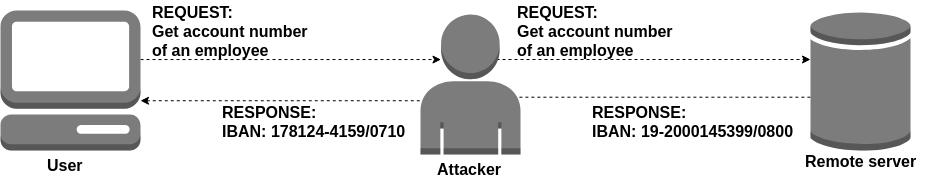
\includegraphics[width=1.0\textwidth]{obrazky-figures/unsecureconnection.png}
        \caption{Example of unauthorised data access and modification during its transmission.}
    \end{center}
\end{figure}

Usage of cryptography is the most frequently used solution for this problem. Data can be encrypted during the communication or encrypted data can be stored on servers and then transferred with or without further encryptions. This thesis will use the second approach, where data are already encrypted on a remote server. Under the term of data, you can imagine usual web page including not only text, images or videos but javascript and CSS as well. Some elements of this page (or even whole page) can be encrypted using an symmetric cypher and different parts can be encrypted using a different key or some parts can be encrypted using multiple keys. These keys are encrypted with asymmetric cypher and they are part of encrypted content as well. The outcome of this thesis will be a web browser extension that will be able to detect encrypted content (images, videos, text, etc.) and decrypt it for a user using his available keys. With this encryption/decryption system, users can create web pages where different data can be accessible for different users without the need for authentication on a remote server.

The target platform will be GNU/Linux and web extensions will be implemented for Firefox browser. Data will be decrypted with the Linux command line application called gpg, that will be used not only for decryption but for key management as well.

\chapter{Theory}
To develop functional and sufficient software for decrypting web pages, it is necessary to understand the tools we will work with. The purpose of this chapter is to introduce you to used technology in this thesis, such as GnuPG or WebExtensions. These tools have their advantages, disadvantages, and limits.

\section{The GNU Privacy Guard}
The GNU Privacy Guard, also known as GnuPG or GPG, is a complete and free implementation of the OpenPGP standard as defined by RFC4880. GnuPG offers encryption, decryption and signing both data and communication. It features a versatile key management system with access modules for many kinds of public key directories. Not only that GnuPG is available for both Windows and Linux, but also a wealth of applications and libraries are available.
%https://gnupg.org/

Linux implementation of GnuPG is a command line tool with features for integration with other applications. Windows version of GnuPG is Gpg4win with a context menu tool, a crypto manager, and an Outlook plugin to send and receive standard PGP/MIME mails.
%https://gnupg.org/

\subsection{OpenPGP standard}
As mentioned earlier, GnuPG is the implementation of OpenPGP standard. OpenPGP combines symmetric-key encryption and public-key encryption to provide confidentiality.   Firstly the object is encrypted using a symmetric encryption algorithm. It is worth mentioning that each symmetric key is used only once for a single object. For each object, a new key is generated as a random number. This key is bound to the message and transmitted with it. Key is protected by encryption as well - the key is encrypted with the receiver's public key. The sequence is as follows:
\begin{enumerate}
    \item The sender creates a message.
    \item The sending OpenPGP generates a random number to be used as a session key for this message only.
    \item The generated session key is encrypted using each recipient's public key. These encrypted session keys start the message.
    \item The sending OpenPGP encrypts the message using the session key, which forms the remainder of the message. Note that the message is also usually compressed.
    \item The receiving OpenPGP decrypts the session key using the recipient's private key.
    \item The receiving OpenPGP decrypts the message using the session key. If the message was compressed, it will be decompressed.
\end{enumerate}
% https://www.ietf.org/rfc/rfc4880.txt

A symmetric key, that is used for message encryption, can be derived from a passphrase (or different kind of shared secret), or a two-stage mechanism similar to the public-key method that was described above in which a session key is itself encrypted with a symmetric algorithm keyed from a shared secret.
%https://www.ietf.org/rfc/rfc4880.txt

Authentication can be achieved using a digital signature. The digital signature uses a hash code or message digest algorithm, and a public-key signature algorithm. The sequence is as follows:
\begin{enumerate}
    \item A message is created by the sender.
    \item The sending software generates a hash code of the message.
    \item The sending software generates a signature from the hash code using the sender's private key.
    \item The binary signature is attached to the message.
    \item The receiving software keeps a copy of the message signature.
    \item The receiving software generates a new hash code for the received message and verifies it using the message's signature.
\end{enumerate}
% https://www.ietf.org/rfc/rfc4880.txt

Both confidentiality and signature services may be applied to the same message. First signature is created and attached to the message. Then message (including signature) is encrypted using a symmetric session key. At last, this session key is encrypted with public-key encryption and prefixed to the encrypted message.
% https://www.ietf.org/rfc/rfc4880.txt

\section{Browser Extensions}

\chapter{Draft and Implementation}

\chapter{Conclusion}
